\chapter{Datasets and MonteCarlo samples}
\label{ch:samples}

% **************************** Define Graphics Path **************************
\ifpdf
    \graphicspath{{Chapter5_2/Figs/Raster/}{Chapter5_2/Figs/PDF/}{Chapter5_2/Figs/}}
\else
    \graphicspath{{Chapter5_2/Figs/Vector/}{Chapter5_2/Figs/}}
\fi

\section{Datasets}

The datasets used in this analysis are listed in Table~\ref{tab:datasets}, each containing
events from a specific trigger of interest. The primary 
signal samples are named `HTMHTParked', spanning over the 2012 run periods B, C and D,
with a total combined integrated luminosity of 18.49~\fb. Control samples used for
predictions of SM backgrounds include `JetHT', `SingleMu' and `SinglePhoton', covering 
run periods A, B, C and D, with
combined integrated luminosities of 18.48~\fb, 19.13~\fb and 19.12~\fb, respectively.

\begin{table}[ht]
\caption{8 \tev Datasets with the integrated luminosity for each.}
  \label{tab:datasets}
  \centering
  \scriptsize
  \begin{tabular}{ lc }
    \hline
    \hline
    Dataset & Luminosity (fb$^{-1}$) \\
    \hline
    \verb!/HTMHTParked/Run2012B-22Jan2013-v1/AOD! & 4.41 \\
    \verb!/HTMHTParked/Run2012C-22Jan2013-v1/AOD! & 6.80 \\
    \verb!/HTMHTParked/Run2012D-22Jan2013-v1/AOD! & 7.29 \\
    \multicolumn{1}{r}{Total} & 18.49 \\ [0.5ex]
    % \verb!/HT/Run2012A-22Jan2013-v1/AOD! & n/a \\
    \verb!/JetHT/Run2012B-22Jan2013-v1/AOD! & 4.39 \\
    \verb!/JetHT/Run2012C-22Jan2013-v1/AOD! & 6.80 \\
    \verb!/JetHT/Run2012D-22Jan2013-v1/AOD! & 7.29 \\
    \multicolumn{1}{r}{Total} & 18.48 \\ [0.5ex]
    \verb!/SingleMu/Run2012A-22Jan2013-v1/AOD! & 0.69 \\
    \verb!/SingleMu/Run2012B-22Jan2013-v1/AOD! & 4.40 \\
    \verb!/SingleMu/Run2012C-22Jan2013-v1/AOD! & 6.77 \\
    \verb!/SingleMu/Run2012D-22Jan2013-v1/AOD! & 7.27 \\
    \multicolumn{1}{r}{Total} & 19.13 \\ [0.5ex] % 19.13
    \verb!/Photon/Run2012A-22Jan2013-v1/AOD! & 0.68 \\
    \verb!/SinglePhoton/Run2012B-22Jan2013-v1/AOD! & 4.40 \\
    \verb!/SinglePhoton/Run2012C-22Jan2013-v1/AOD! & 6.77 \\
    \verb!/SinglePhotonParked/Run2012D-22Jan2013-v1/AOD! & 7.27 \\
    \multicolumn{1}{r}{Total} & 19.12 \\ [0.5ex] % 19.18
    \hline
    \hline
  \end{tabular}
\end{table}

\section{MonteCarlo Background and Signal samples}

The full set of simulated MonteCarlo (MC) samples used in this analysis are listed in 
Table~\ref{tab:mc-sm} along with the number of events, next-to-next-to-leading 
order (NNLO) cross section and an effective integrated luminosity for each. These
samples contain simulated events of relevant sources of SM backgrounds, specifically
\ttbar, photon, W boson and Z boson production, each with associated jets, as well as
dedicated samples of QCD production. 

The Parton Density Function (PDF) of colliding protons are modelled according
to the
CTEQ6L1 distribution~\cite{Pumplin:2002vw}, the matrix-element level hard-scatter
performed by
\MADGRAPHFIVE~\cite{Alwall:2007st}, \POWHEGONE~\cite{Alioli:2010xd} or \PYTHIASIX~\cite{Sjostrand:2000wi}, with
outgoing partons showered in \PYTHIASIX. The
produced generator level particles are then input into a full detector
simulation in \GEANTFOUR~\cite{Agostinelli2003250}, and detector hits `digitized'
in order to simulate the response of detector electronics. Prior to digitization, a number of
`MinimumBias' events are overlayed in order to reproduce LHC run conditions. Event-level weights
are applied to each simulated sample such that both the PU and equivalent
integrated luminosity are matched to a given data sample.

Additional corrections are made to simulated event samples in order to correct
the efficiency of b tagging algorithms to match that observed in data.
Corrections are determined as a function of jet-flavour (light/c/b), defined as:
% 
\begin{equation}
SF_{light,c,b} = \frac{\epsilon^{data}_{light,c,b}(\Pt, \eta)}{\epsilon^
{MC}_ {light,c,b}(\Pt, \eta)} ,
\label{eq:btag_scalefactor}
\end{equation}
% 
where $\epsilon^{data}_{light, c, b}$ and $\epsilon^{MC}_{light, c, b}$ represent \Pt and $\eta$ dependent
b tagging efficiencies measured in data and MC respectively. These are calculated and provided
centrally by the BTAG \emph{POG}~\cite{btagpog-scalefactors}.

\begin{landscape}
  \begin{center}
    \begin{table}[ht]
      \caption{MC samples for Standard Model processes with their NNLO cross
      sections and equivalent integrated luminosity.}
      \label{tab:mc-sm}
      \centering
      \tiny
      \begin{tabular}{ lrrrr }
        \hline
        Sample & N$_{\textrm{event}}$ & Cross section (pb) & Corrected Cross section (pb) & Luminosity (fb$^{-1}$) \\
        \hline
        \hline
        \verb!/WJetsToLNu_TuneZ2Star_8TeV-madgraph-tarball/Summer12_DR53X-PU_S10_START53_V7A-v1/AODSIM!           & 57661905 & 37509.0 & 34133.2 & 1.5     \\
        \verb!/WJetsToLNu_HT-150To200_8TeV-madgraph/Summer12_DR53X-PU_S10_START53_V7C-v1/AODSIM!                  & 21414209 & 253.8   & 234.53  & 84.4    \\
        \verb!/WJetsToLNu_HT-200To250_8TeV-madgraph/Summer12_DR53X-PU_S10_START53_V7C-v1/AODSIM!                  & 9895771  & 116.5   & 103.94  & 84.9    \\
        \verb!/WJetsToLNu_HT-250To300_8TeV-madgraph_v2/Summer12_DR53X-PU_S10_START53_V7A-v1/AODSIM!               & 4924990  & 57.6    & 51.34   & 85.5    \\
        \verb!/WJetsToLNu_HT-300To400_8TeV-madgraph_v2/Summer12_DR53X-PU_S10_START53_V7A-v1/AODSIM!               & 5141023  & 48.4    & 42.41   & 106.2   \\
        \verb!/WJetsToLNu_HT-400ToInf_8TeV-madgraph_v2/Summer12_DR53X-PU_S10_START53_V7A-v1/AODSIM!               & 4923847  & 30.8    & 26.36   & 159.9   \\
        \verb!/ZJetsToNuNu_50_HT_100_TuneZ2Star_8TeV_madgraph(_ext)/Summer12_DR53X-PU_S10_START53_V7A-v1/AODSIM!  & 23743998 & 452.8   & 405.21  & 52.4    \\
        \verb!/ZJetsToNuNu_100_HT_200_TuneZ2Star_8TeV_madgraph(_ext)/Summer12_DR53X-PU_S10_START53_V7A-v1/AODSIM! & 9876059  & 190.4   & 173.76  & 51.9    \\
        \verb!/ZJetsToNuNu_200_HT_400_TuneZ2Star_8TeV_madgraph(_ext)/Summer12_DR53X-PU_S10_START53_V7A-v1/AODSIM! & 9649619  & 45.1    & 42.41   & 214.0   \\
        \verb!/ZJetsToNuNu_400_HT_inf_TuneZ2Star_8TeV_madgraph(_ext)/Summer12_DR53X-PU_S10_START53_V7A-v1/AODSIM! & 5079710  & 6.26    & 5.81    & 811.5   \\
        \verb!/TT_CT10_TuneZ2star_8TeV-powheg-tauola/Summer12_DR53X-PU_S10_START53_V7A-v1(v2)/AODSIM!             & 27094723 & 234.0   & 271.44  & 115.8   \\
        \verb!/TTZJets_8TeV-madgraph_v2/Summer12_DR53X-PU_S10_START53_V7A-v1/AODSIM!                              & 210160   & 0.172   & 0.172   & 1221.9  \\
        \verb!/TTWJets_8TeV-madgraph/Summer12_DR53X-PU_S10_START53_V7A-v1/AODSIM!                                 & 182327   & 0.2149  & 0.2149  & 848.4   \\
        \verb!/T_t-channel_TuneZ2star_8TeV-powheg-tauola/Summer12_DR53X-PU_S10_START53_V7A-v1/AODSIM!             & 3710227  & 56.4    & 56.4    & 65.8    \\
        \verb!/Tbar_t-channel_TuneZ2star_8TeV-powheg-tauola/Summer12_DR53X-PU_S10_START53_V7A-v1/AODSIM!          & 1935072  & 30.7    & 30.7    & 63.0    \\
        \verb!/T_s-channel_TuneZ2star_8TeV-powheg-tauola/Summer12_DR53X-PU_S10_START53_V7A-v1/AODSIM!             & 243961   & 3.79    & 3.79    & 64.4    \\
        \verb!/Tbar_s-channel_TuneZ2star_8TeV-powheg-tauola/Summer12_DR53X-PU_S10_START53_V7A-v1/AODSIM!          & 139974   & 1.76    & 1.76    & 79.5    \\
        \verb!/T_tW-channel-DR_TuneZ2star_8TeV-powheg-tauola/Summer12_DR53X-PU_S10_START53_V7A-v1/AODSIM!         & 497658   & 11.1    & 11.1    & 44.8    \\
        \verb!/Tbar_tW-channel-DR_TuneZ2star_8TeV-powheg-tauola/Summer12_DR53X-PU_S10_START53_V7A-v1/AODSIM!      & 493460   & 11.1    & 11.1    & 44.5    \\
        \verb!/DYJetsToLL_M-10To50filter_8TeV-madgraph/Summer12_DR53X-PU_S10_START53_V7A-v1/AODSIM!               & 7116223  & 13124.1 & 12205.4 & 0.5     \\
        \verb!/DYJetsToLL_M-50_TuneZ2Star_8TeV-madgraph-tarball/Summer12_DR53X-PU_S10_START53_V7A-v1/AODSIM!      & 30171503 & 3503.7  & 3258.45 & 8.6     \\
        \verb!/DYJetsToLL_HT-200To400_TuneZ2Star_8TeV-madgraph(_ext)/Summer12_DR53X-PU_S10_START53_V7A-v1/AODSIM! & 6892777  & 24.3    & 22.24   & 283.7   \\
        \verb!/DYJetsToLL_HT-400ToInf_TuneZ2Star_8TeV-madgraph/Summer12_DR53X-PU_S10_START53_V7A-v1/AODSIM!       & 2695789  & 3.36    & 3.11    & 802.3   \\
        \verb!/GJets_HT-200To400_8TeV-madgraph/Summer12_DR53X-PU_S10_START53_V7A-v1/AODSIM!                       & 57891147 & 1140.8  & 1060.9  & 50.7    \\
        \verb!/GJets_HT-400ToInf_8TeV-madgraph/Summer12_DR53X-PU_S10_START53_V7A-v1/AODSIM!                       & 9459562  & 124.7   & 115.97  & 75.9    \\
        \verb!/WW_TuneZ2star_8TeV_pythia6_tauola/Summer12_DR53X-PU_S10_START53_V7A-v1/AODSIM!                     & 9888431  & 57.1    & 57.1    & 173.2   \\
        \verb!/WZ_TuneZ2star_8TeV_pythia6_tauola/Summer12_DR53X-PU_S10_START53_V7A-v1/AODSIM!                     & 9841248  & 12.6    & 12.6    & 781.1   \\
        \verb!/ZZ_TuneZ2star_8TeV_pythia6_tauola/Summer12_DR53X-PU_S10_START53_V7A-v1/AODSIM!                     & 9751908  & 8.26    & 8.26    & 1180.6  \\
        \verb!/QCD_Pt-50to80_TuneZ2star_8TeV_pythia6/Summer12_DR53X-PU_S10_START53_V7A-v2!                        & 5950860  & 8148778 (LO) & 8148778 (LO) & 0.001   \\
        \verb!/QCD_Pt-80to120_TuneZ2star_8TeV_pythia6/Summer12_DR53X-PU_S10_START53_V7A-v3!                       & 5962864  & 1033680 (LO) & 1033680 (LO) & 0.006   \\
        \verb!/QCD_Pt-120to170_TuneZ2star_8TeV_pythia6/Summer12_DR53X-PU_S10_START53_V7A-v3!                      & 5985732  & 156293 (LO)  & 156293  (LO) & 0.038   \\
        \verb!/QCD_Pt-170to300_TuneZ2star_8TeV_pythia6/Summer12_DR53X-PU_S10_START53_V7A-v1(v2)!                  & 20155180 & 34138 (LO)   & 34138   (LO) & 0.590   \\
        \verb!/QCD_Pt-300to470_TuneZ2star_8TeV_pythia6/Summer12_DR53X-PU_S10_START53_V7A-v1(v2,v3)!               & 23588100 & 1759.5 (LO)  & 1759.5  (LO) & 13.4    \\
        \verb!/QCD_Pt-470to600_TuneZ2star_8TeV_pythia6/Summer12_DR53X-PU_S10_START53_V7A-v2!                      & 3978848  & 113.9 (LO)   & 113.9   (LO) & 34.9    \\
        \verb!/QCD_Pt-600to800_TuneZ2star_8TeV_pythia6/Summer12_DR53X-PU_S10_START53_V7A-v2!                      & 3964864  & 27.0 (LO)    & 27.0    (LO) & 146.8   \\
        \verb!/QCD_Pt-800to1000_TuneZ2star_8TeV_pythia6/Summer12_DR53X-PU_S10_START53_V7A-v2!                     & 3854563  & 3.55 (LO)   & 3.55    (LO) & 1085.8  \\
        \verb!/QCD_Pt-1000to1400_TuneZ2star_8TeV_pythia6/Summer12_DR53X-PU_S10_START53_V7A-v1!                    & 1964088  & 0.738 (LO)   & 0.738   (LO) & 2661.4  \\
        \verb!/QCD_Pt-1400to1800_TuneZ2star_8TeV_pythia6/Summer12_DR53X-PU_S10_START53_V7A-v1!                    & 1988062  & 0.0335 (LO)  & 0.0335  (LO) & 59345.1 \\
        \verb!/QCD_Pt-1800_TuneZ2star_8TeV_pythia6/Summer12_DR53X-PU_S10_START53_V7A-v1!                          & 977586   & 0.00183 (LO) & 0.00183 (LO) & 534200  \\
        \verb!/QCD_HT-100To250_TuneZ2star_8TeV-madgraph-pythia/Summer12_DR53X-PU_S10_START53_V7A-v1/AODSIM!       & 50081518 & 1.036E7 (LO) & 1.036E7 (LO) & 0.005   \\
        \verb!/QCD_HT-250To500_TuneZ2star_8TeV-madgraph-pythia6/Summer12_DR53X-PU_S10_START53_V7A-v1/AODSIM!      & 27062078 & 276000 (LO) & 276000 (LO) & 0.1     \\
        \verb!/QCD_HT-500To1000_TuneZ2star_8TeV-madgraph-pythia6/Summer12_DR53X-PU_S10_START53_V7A-v1/AODSIM!     & 27613225 & 8426 (LO)   & 8426   (LO) & 3.3     \\
        \verb!/QCD_HT-1000ToInf_TuneZ2star_8TeV-madgraph-pythia6/Summer12_DR53X-PU_S10_START53_V7A-v1/AODSIM!     & 12018415 & 204 (LO)    & 204    (LO) & 58.9    \\
        \hline
      \end{tabular}
    \end{table}
  \end{center}
\end{landscape}

Interpretations are made using signal MC samples, each representing a scan in 
the phase space of a specific SMS model. These samples are listed in
Table~\ref{tab:mc-signal}. Each sample is generated at the parton level using \MADGRAPHFIVE and then
decayed using \PYTHIASIX. Diagrams for up to two additional
partons are simulated
in the initial generation step to ensure good modelling of initial state 
radiation (ISR), however supplementary samples were produced with up to three
additional partons to allow for systematic studies into the effect on 
analysis acceptance, as detailed in chapter~\ref{ch:interpretation}.

Signal MC samples use the \FASTSIM detector simulation framework~\cite{1742-6596-513-2-022012}
in order to simulate detector and electronics responses. In comparison to the
\FULLSIM method used for all other MC backgrounds, \FASTSIM aims to greatly
reduce the processing time required to generate samples by avoiding the
CPU-intensive full detector simulation of the \GEANT framework, instead
employing detector response parametrisations tuned using \FULLSIM samples.

\begin{landscape}
  \begin{center}
    \begin{table}[ht]
      \caption{MC samples for Simplified Model Spectra.}
      \label{tab:mc-signal}
      \centering
      \tiny
      \begin{tabular}{ lll }
        \hline
        Model & Sample & Description \\
        \hline
        \hline
        \verb!Charm decay!     & \verb!/SMS-MadGraph_2J_T2cc_NoFilter_mStop-100to250_mLSP-20to230_8TeV-Pythia6Zstar/Summer12-START52_V9_FSIM-v1/AODSIM! & Original scan \\
        \verb!Charm decay!     & \verb!/SMS-T2cc_NoFilter_mStop-175to250_mLSP-95to240_8TeV-Pythia6Z/Summer12-START52_V9_FSIM-v1/AODSIM! & Original scan \\
        \verb!Charm decay!     & \verb!/SMS-T2cc_2J_mStop-250to350_mLSP-195to340_TuneZ2star_8TeV-madgraph-tauola/Summer12-START53_V19_FSIM-v2/AODSIM! & Scan extension \\
        \verb!Charm decay!     & \verb!/SMS-8TeV_Pythia6Z_T2cc_3jets_mStop-200_mLSP-120/Summer12-START52_V9_FSIM-v1/AODSIM! & 3-parton sample \\
        \verb!Charm decay!     & \verb!/SMS-8TeV_Pythia6Z_T2cc_3jets_mStop-200_mLSP-190/Summer12-START52_V9_FSIM-v1/AODSIM! & 3-parton sample \\
        \verb!Four-body decay! & \verb!/SMS-T2DegenerateStop_2J_mStop-100to150_mLSP-20to140_TuneZ2star_8TeV-madgraph-tauolapp/Summer12-START53_V19_FSIM_PU_S12-v1/AODSIM! & Original scan \\
        \verb!Four-body decay! & \verb!/SMS-T2DegenerateStop_2J_mStop-175to225_mLSP-95to215_TuneZ2star_8TeV-madgraph-tauolapp/Summer12-START53_V19_FSIM_PU_S12-v1/AODSIM! & Original scan \\
        \verb!Four-body decay! & \verb!/SMS-T2DegenerateStop_2J_mStop-250to300_mLSP-170to290_TuneZ2star_8TeV-madgraph-tauolapp/Summer12-START53_V19_FSIM_PU_S12-v1/AODSIM! & Original scan \\
        \verb!Four-body decay! & \verb!/SMS-T2DegenerateStop_2J_mStop-325to375_mLSP-245to365_TuneZ2star_8TeV-madgraph-tauolapp/Summer12-START53_V19_FSIM_PU_S12-v1/AODSIM! & Original scan \\
        \verb!Four-body decay! & \verb!/SMS-T2DegenerateStop_2J_mStop-400_mLSP-320to390_TuneZ2star_8TeV-madgraph-tauolapp/Summer12-START53_V19_FSIM_PU_S12-v1/AODSIM! & Original scan \\
        \hline
        \hline
      \end{tabular}
    \end{table}
  \end{center}
\end{landscape}

\section{Correcting SM sample cross sections}
\label{sec:mc_xsec_corrs}

\subsection{\HTpart binned samples}
Given the computing resources required to produce MC samples, statistics
can be greatly increased by only simulating events within some kinematic range.
This analysis therefore makes use of MC samples binned
according to parton-level \HT (\HTpart - the scalar sum of transverse energies of 
the quarks and gluons involved in the hard scatter process). The binned samples
correspond to the processes \wj, \zj and \dyj.
Leading order (LO) cross-sections are provided with 
these samples, which are translated into next-to-next-to-leading order (NNLO) 
cross-sections using scaling-factors (k-factors) derived from corresponding 
inclusive sample cross-sections (where $k = \sigma_{NNLO}/\sigma_{LO})$. However,
recent CMS studies~\cite{RobXS} have shown that the
provided LO cross-sections for \HTpart binned samples can 
be incorrect by up to 10\%. To ensure \HTpart binned samples are fully consistent
with their corresponding inclusive samples, the following procedure is used:

\begin{enumerate}
\item Calculate the $\sigma_{NNLLO}$ for each \HTpart binned sample using k-factors derived from inclusive samples.
In the case of \zj where no such inclusive sample exists, k-factors are taken from the \dyj sample.
\item Compare the distribution of \HTpart between the binned and inclusive samples. Again, \zj binned is compared to \dyj inclusive.
\item Derive corrections to $\sigma_{NNLO}$ for each \HTpart sample such that the ratio between the \HTpart distributions
is 1.0, or in the case of \zj vs. \dyj, the ratio of the PDG measured cross-sections, 0.505~\cite{Agashe:2014kda}.
\end{enumerate}

\begin{figure}[b!]
  \centering
  \begin{subfigure}[b]{0.48\textwidth}
    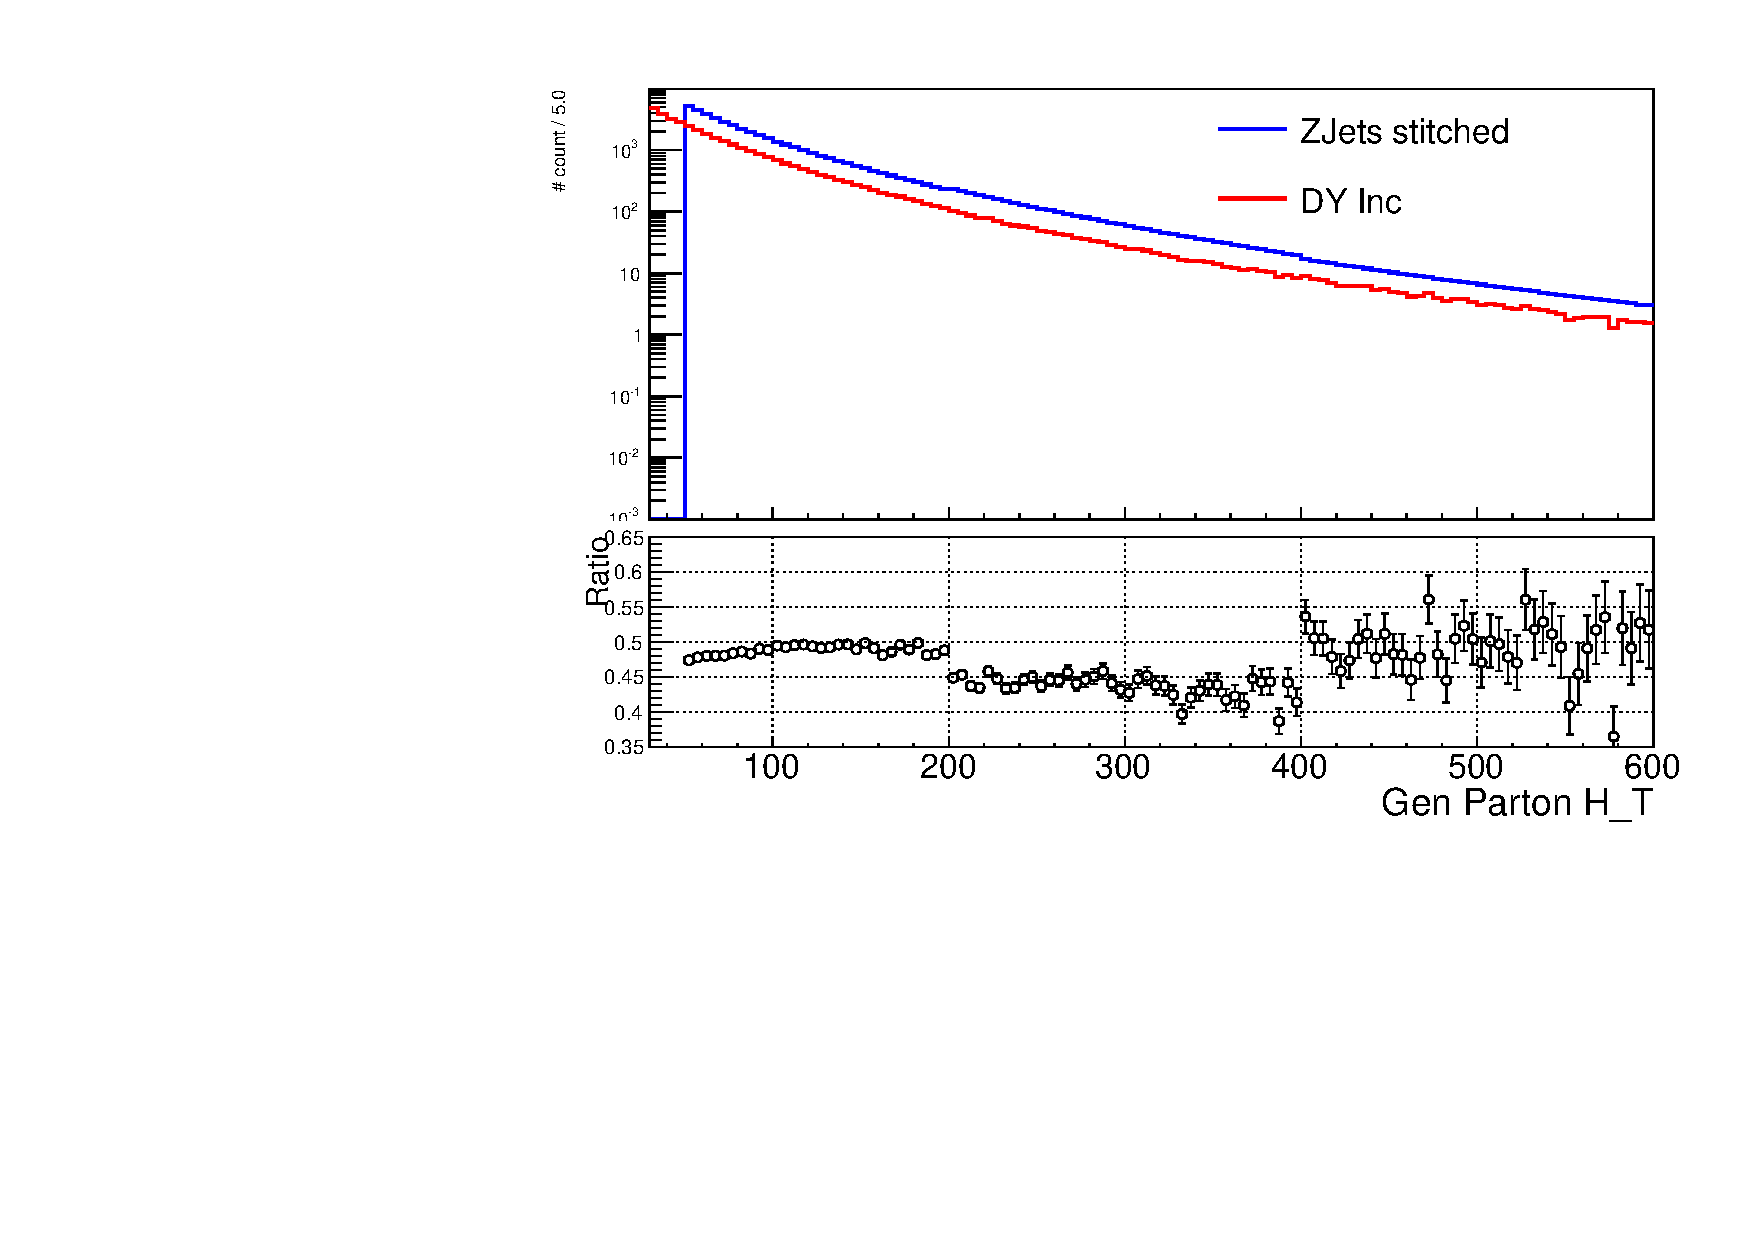
\includegraphics[width=\textwidth]{/Users/chrislucas/SUSY/thesis/Figs/xs_study/compar_genPartonHT_zmass_0_inc_inc_DYZJets_noCuts_sitv_log_HCPxS.pdf}
    \caption{No corrections.}
    \label{fig:xsec_study_before}
  \end{subfigure}             
  \begin{subfigure}[b]{0.48\textwidth}
    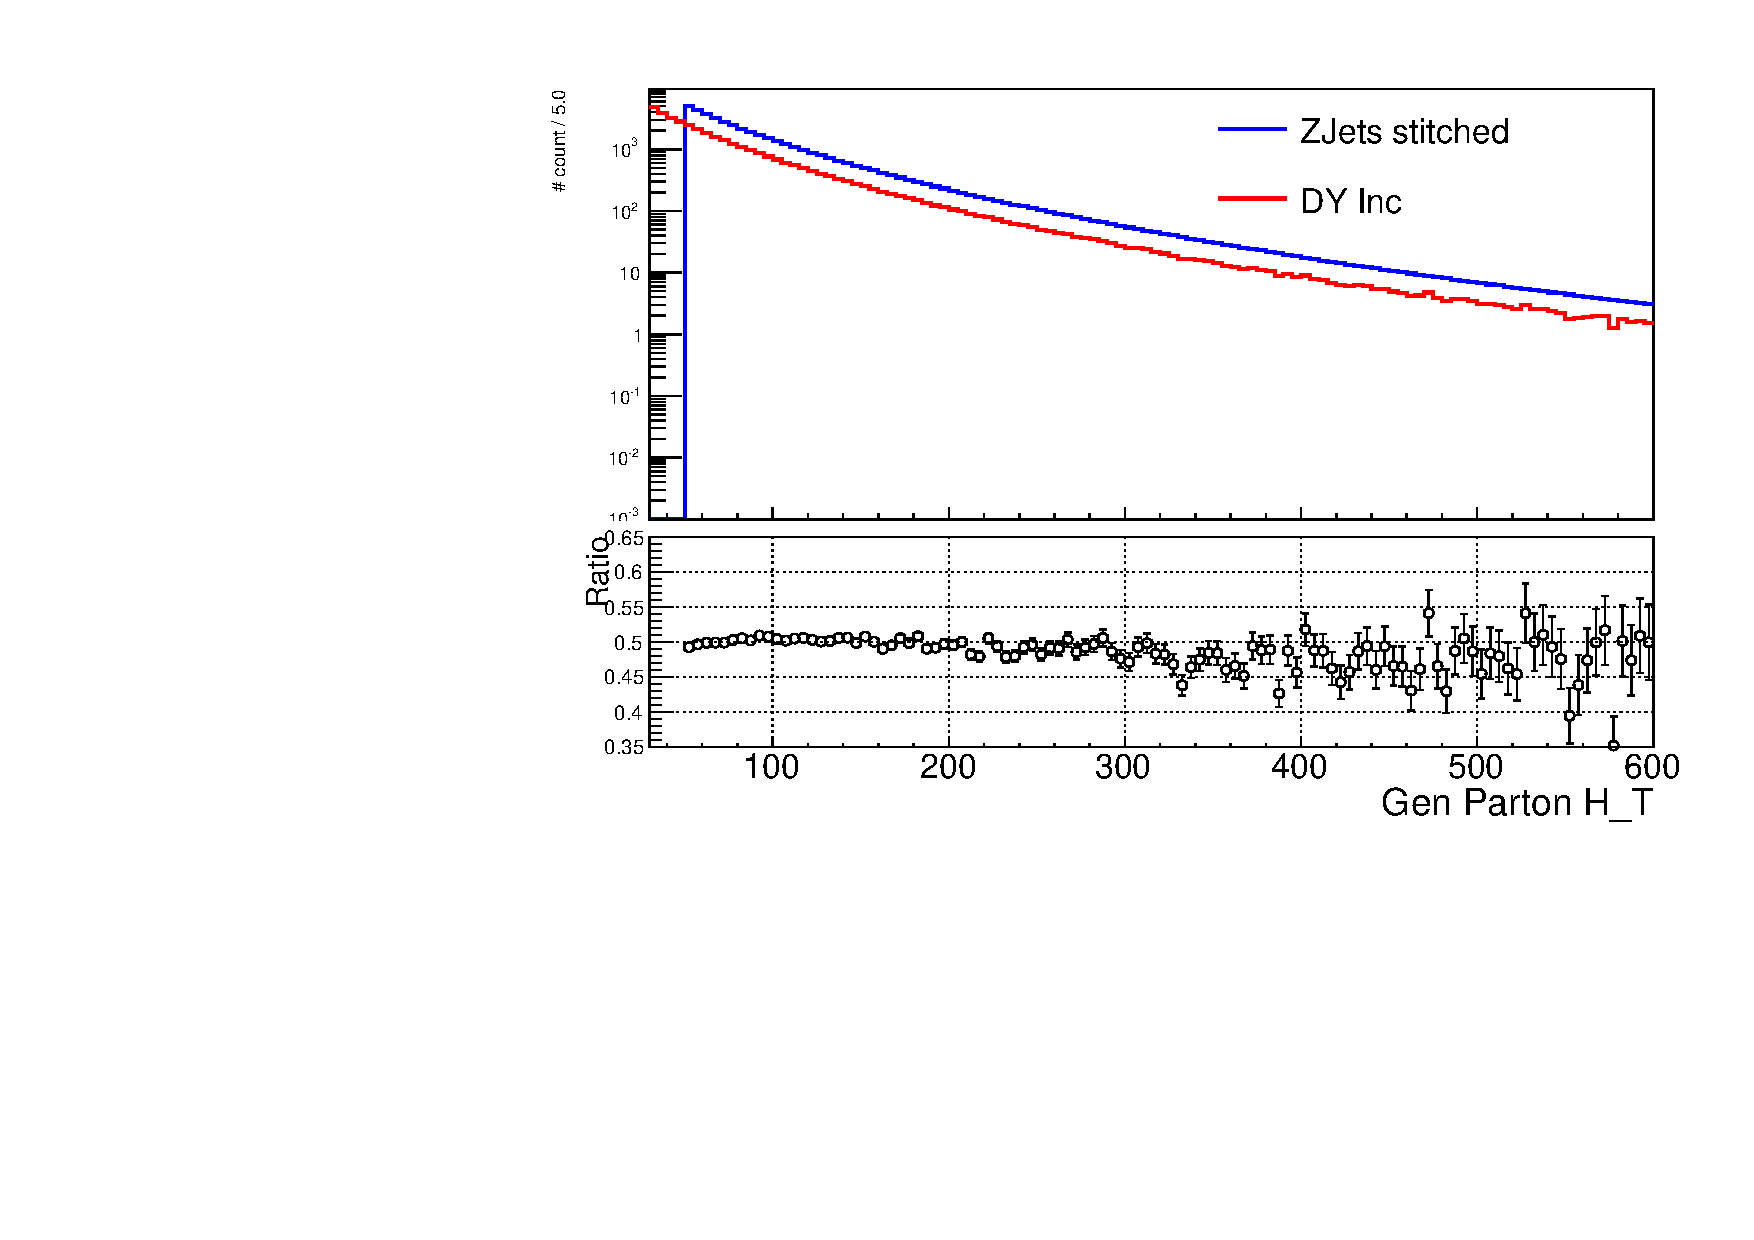
\includegraphics[width=\textwidth]{/Users/chrislucas/SUSY/thesis/Figs/xs_study/compar_genPartonHT_zmass_0_inc_inc_DYZJets_noCuts_sitv_log.pdf}
    \caption{With corrections.}
    \label{fig:xsec_study_after}
  \end{subfigure}             
  \caption{Generator level \HTpart distributions from the
    inclusive DY + jets and the \HTpart binned \zj
    samples, both before and after cross section corrections.}
  \label{fig:xsec_study}
\end{figure}

Example \HTpart distributions before and after this procedure are shown in
Figure~\ref{fig:xsec_study}, where steps are clearly visible in the
ratio prior to the corrections, and then removed following corrections.


\subsection{\HT sideband normalisation}

As mentioned in Section~\ref{sec:mc_xsec_corrs}, absolute MC 
normalisation is not well modelled in the high-\met region of 
phase-space in which many SUSY analyses search. As such, data and MC are seen to
disagree when using standard MC samples and cross-sections. While data and MC
comparisons are not explicitly used in this analysis, ratios of MC yields are, 
and so cross-section correction factors for the main 
MC samples must be derived. Corrections are taken as the data to MC ratio
in the $150 \leq \HT < 200$~\gev sideband region. For the three main EWK backgrounds,
\wj, \zj and \ttbar + jets, a particular combination of control region selection (control regions described
later in chapter~\ref{ch:background}), jet and b-tagged jet multiplicity, is used to ensure
a pure selection of a given process. The selections and their purities are listed in 
Table~\ref{tab:ht_sideband}. Also listed are the derived correction factors to
be applied to MC, indicating the level of disagreement present between data and MC
observed in the sideband region.

\begin{table}[!ht]
  % \caption{Correction factors determined as the ratio of yields in data to
  % those in MC, for a sideband region of $150 < \HT < 200$ \gev. Factors are
  % calculated for process-specific MC samples by choosing a selection enriched in
  % the relevant process, and applied as a global correction.}
  \caption{The process-specific sideband corrections applied to MC sample, with
  the selection used and its corresponding purity.}
  \label{tab:ht_sideband}
  \centering
  \small
  \begin{tabular}{ llcc }
    \hline
    \hline
    Process                       & Selection                         & Purity & Correction factor        \\
    \hline
    W + jets                      & \mj, \njlow, $\nb = 0$          & 0.91   & $0.93 \pm 0.01$ \\
    Z($\rightarrow\mu\mu$) + jets & \mmj, \njlow, $\nb = 0$         & 0.98   & $0.94 \pm 0.04$ \\
%    \ttbar                       & \mj, $\nj \geq 2$, $\nb \geq 2$ & 0.73   & $1.25 \pm 0.05$ \\
    \ttbar                        & \mj, $\nj \geq 2$, $\nb \geq 2$ & 0.87   & $1.21 \pm 0.05$ \\ % includes single top
    \hline
    \hline
  \end{tabular}
\end{table}

The validity of this procedure is ultimately tested using a suite of 
closure tests (discussed in Section~\ref{sec:closure_tests}).

\section{Predicting event yields for high b-jet multiplicities}
\label{sec:formula_method}

Yields taken from the MC samples listed in Table~\ref{tab:mc-sm} are used as input
to the SM background prediction techniques described later in Chapter~\ref{ch:background}.
Given the relatively low number of b tagged jets present in such electroweak
background processes, events containing high b-jet multiplicities (\nb) are
often dominated by mistagged light quarks. Consequently, high-\nb yields often
suffer from a lack of precision due to large statistical uncertainties. In order
to reduce the statistical uncertainties associated with such events, a method has
been developed which considers individual quark-flavour tagging efficiencies and
the underlying quark flavour distribution (both measured directly from
simulation) to determine high-\nb event yields with a greater precision.
This method is employed in this analysis, and while it will not be outlined here,
it is described in detail elsewhere~\cite{an_alphat_hcp_12fb}. 

% Determining yields for analysis categories that require high numbers of b tagged
% jets (\nb) 
% directly from simulation
% becomes
% inherently reliant on not only MC modelling, but also on the underlying physics
% distribution of quark-flavours. For samples of electroweak processes, given the
% abundance of
% low b-jet multiplicity events, high-\nb categories become dominated by
% mistagging of light-flavour jets, leading to large statistical uncertainties.
% In order to reduce statistical uncertainties from directly using MC yields, a method has been
% developed using flavour tagging efficiencies and the underlying quark
% flavour distribution, both measured directly from simulation.

% This `Formula Method' is described in detail elsewhere \cite{an_alphat_hcp_12fb}.

% The approach can be summarised by:
% % 
% \begin{equation}
%   \begin{split}
%   N(n) = \sum_{n_b^{gen} + n_c^{gen} + n_{\text{light}}^{gen} = n_{jet}^{cat}}\:
%   \sum_{n_b^{tag} + n_c^{tag} + n_{\text{light}}^{tag} = n}
%   N(n_b^{gen}, n_c^{gen}, n_q^{gen}) \times \\
%   P(n_b^{tag}, n_b^{gen}, \epsilon_{b}) \times
%   P(n_c^{tag}, n_c^{gen}, \epsilon_{c}) \times
%   P(n_{\text{light}}^{tag}, n_{\text{light}}^{gen}, \epsilon_{\text{light}}) ,
%   \end{split}
% \end{equation}
% % 
% where $N(n)$ represents the predicted yield of $n$ b-tagged events for a
% given
% analysis category and \HT bin. The jet-flavour tagging probability
% terms $P(n_b^{tag}, n_b^{gen}, \epsilon_{b})$,
% $P(n_c^{tag}, n_c^{gen}, \epsilon_{c})$ and 
% $P(n_{\text{light}}^{tag}, n_{\text{light}}^{gen}, \epsilon_{\text{light}})$ are measured for each \HT bin and
% analysis category for each simulated sample, including the flavour tagging
% efficiencies $\epsilon_b$, $\epsilon_c$ and $\epsilon_{\text{light}}$ as also
% measured from
% each sample. Finally, $N(n_b^{gen}, n_c^{gen}, n_q^{gen})$ represents the
% distribution of actual generator-level jet flavours in the events.

% In the large-statistic sample limit this technique would not be necessary,
% as enough high-\nb events would be present to sufficiently reduce statistical
% uncertainties. However, in the absence of this infeasible scenario,
% this technique
% makes uses of all events in a sample, thereby reducing uncertainties
% and ultimately delivering more precise yields from simulation.
